% Prof. Dr. Ausberto S. Castro Vera
% UENF - CCT - LCMAT - Curso de Ci\^{e}ncia da Computa\c{c}\~{a}o
% Campos, RJ,  2023
% Disciplina: Paradigmas de Linguagens de Programa\c{c}\~{a}o
% Aluno: Gabriel Costa Fassarella


\chapterimage{ScalaH} % Chapter heading image
\chapter{Considera\c{c}\~{o}es Finais}
	Ao longo desse livro foram abordados diversos aspectos sobre a linguagem de programação Scala. Inicialmente foi apresentada uma visão geral sobre a linguagem, seguido pela sua história que apesar de ser recente, não existem muitos relatos disponíveis para o público, e por último foram apresentadas algumas aplicações da linguagem no mercado de trabalho. 
	
	Após esse capítulo introdutório, foi abordado durante alguns capítulos aspectos básicos e avançados necessários para a programação em Scala. Em seguida foram demonstradas algumas aplicações utilizando esses conceitos apresentados anteriormente.
	
	É válido lembrar que esse livro foi escrito com o intuito de trazer uma introdução ao Scala junto com alguns necessários para a programação básica na linguagem, com o principal intuito de promover ao leitor o interesse de se aprofundar no estudo da linguagem Scala. 
	Aspectos do Scala que podem ser estudados futuramente:
	\begin{itemize}
		\item Traits e Mixins: Estudar o uso de traits com o objetivo de compartilhar os comportamentos entre classes e como compor traits pode ser algo vantajoso em muitas situações adversas.
		
		\item Programação Assíncrona: Estudar as bibliotecas Promises, Akka e Futures para poder utilizar paralelismo e concorrência de maneira efetiva pode garantir uma ótima eficiência do código.
		
		\item Macros: Estudar a utilização de macros para criar o código em tempo de compilação pode garantir muitas vantagens para o usuário.
		
		\item Implicits: Estudar o uso de implicits com o objetivo de adicionar comportamentos ou tipos implicitamente pode facilitar a utilização de inúmeras bibliotecas.
		
		\item Concorrência e Paralelismo: Como já citado antes, estudar o uso de paralelismo e a concorrência pode aumentar muito a eficiência do código em Scala.
		\end{itemize}

	Portanto, é possível concluir que o Scala é uma linguagem de programação extremamente versátil e útil e diversas áreas diferentes, tanto para o mercado de trabalho quanto para estudo. Isso, junto de sua similaridade com Java faz com que sua utilização tenha aumentado cada vez mais entre os programadores. Por isso, caso o leitor tenha o interesse em continuar ou reforçar os estudos na linguagem, são recomendados os seguintes livros:
	

   \begin{figure}[H]
    \begin{center}
        \caption{} \label{ling2}
        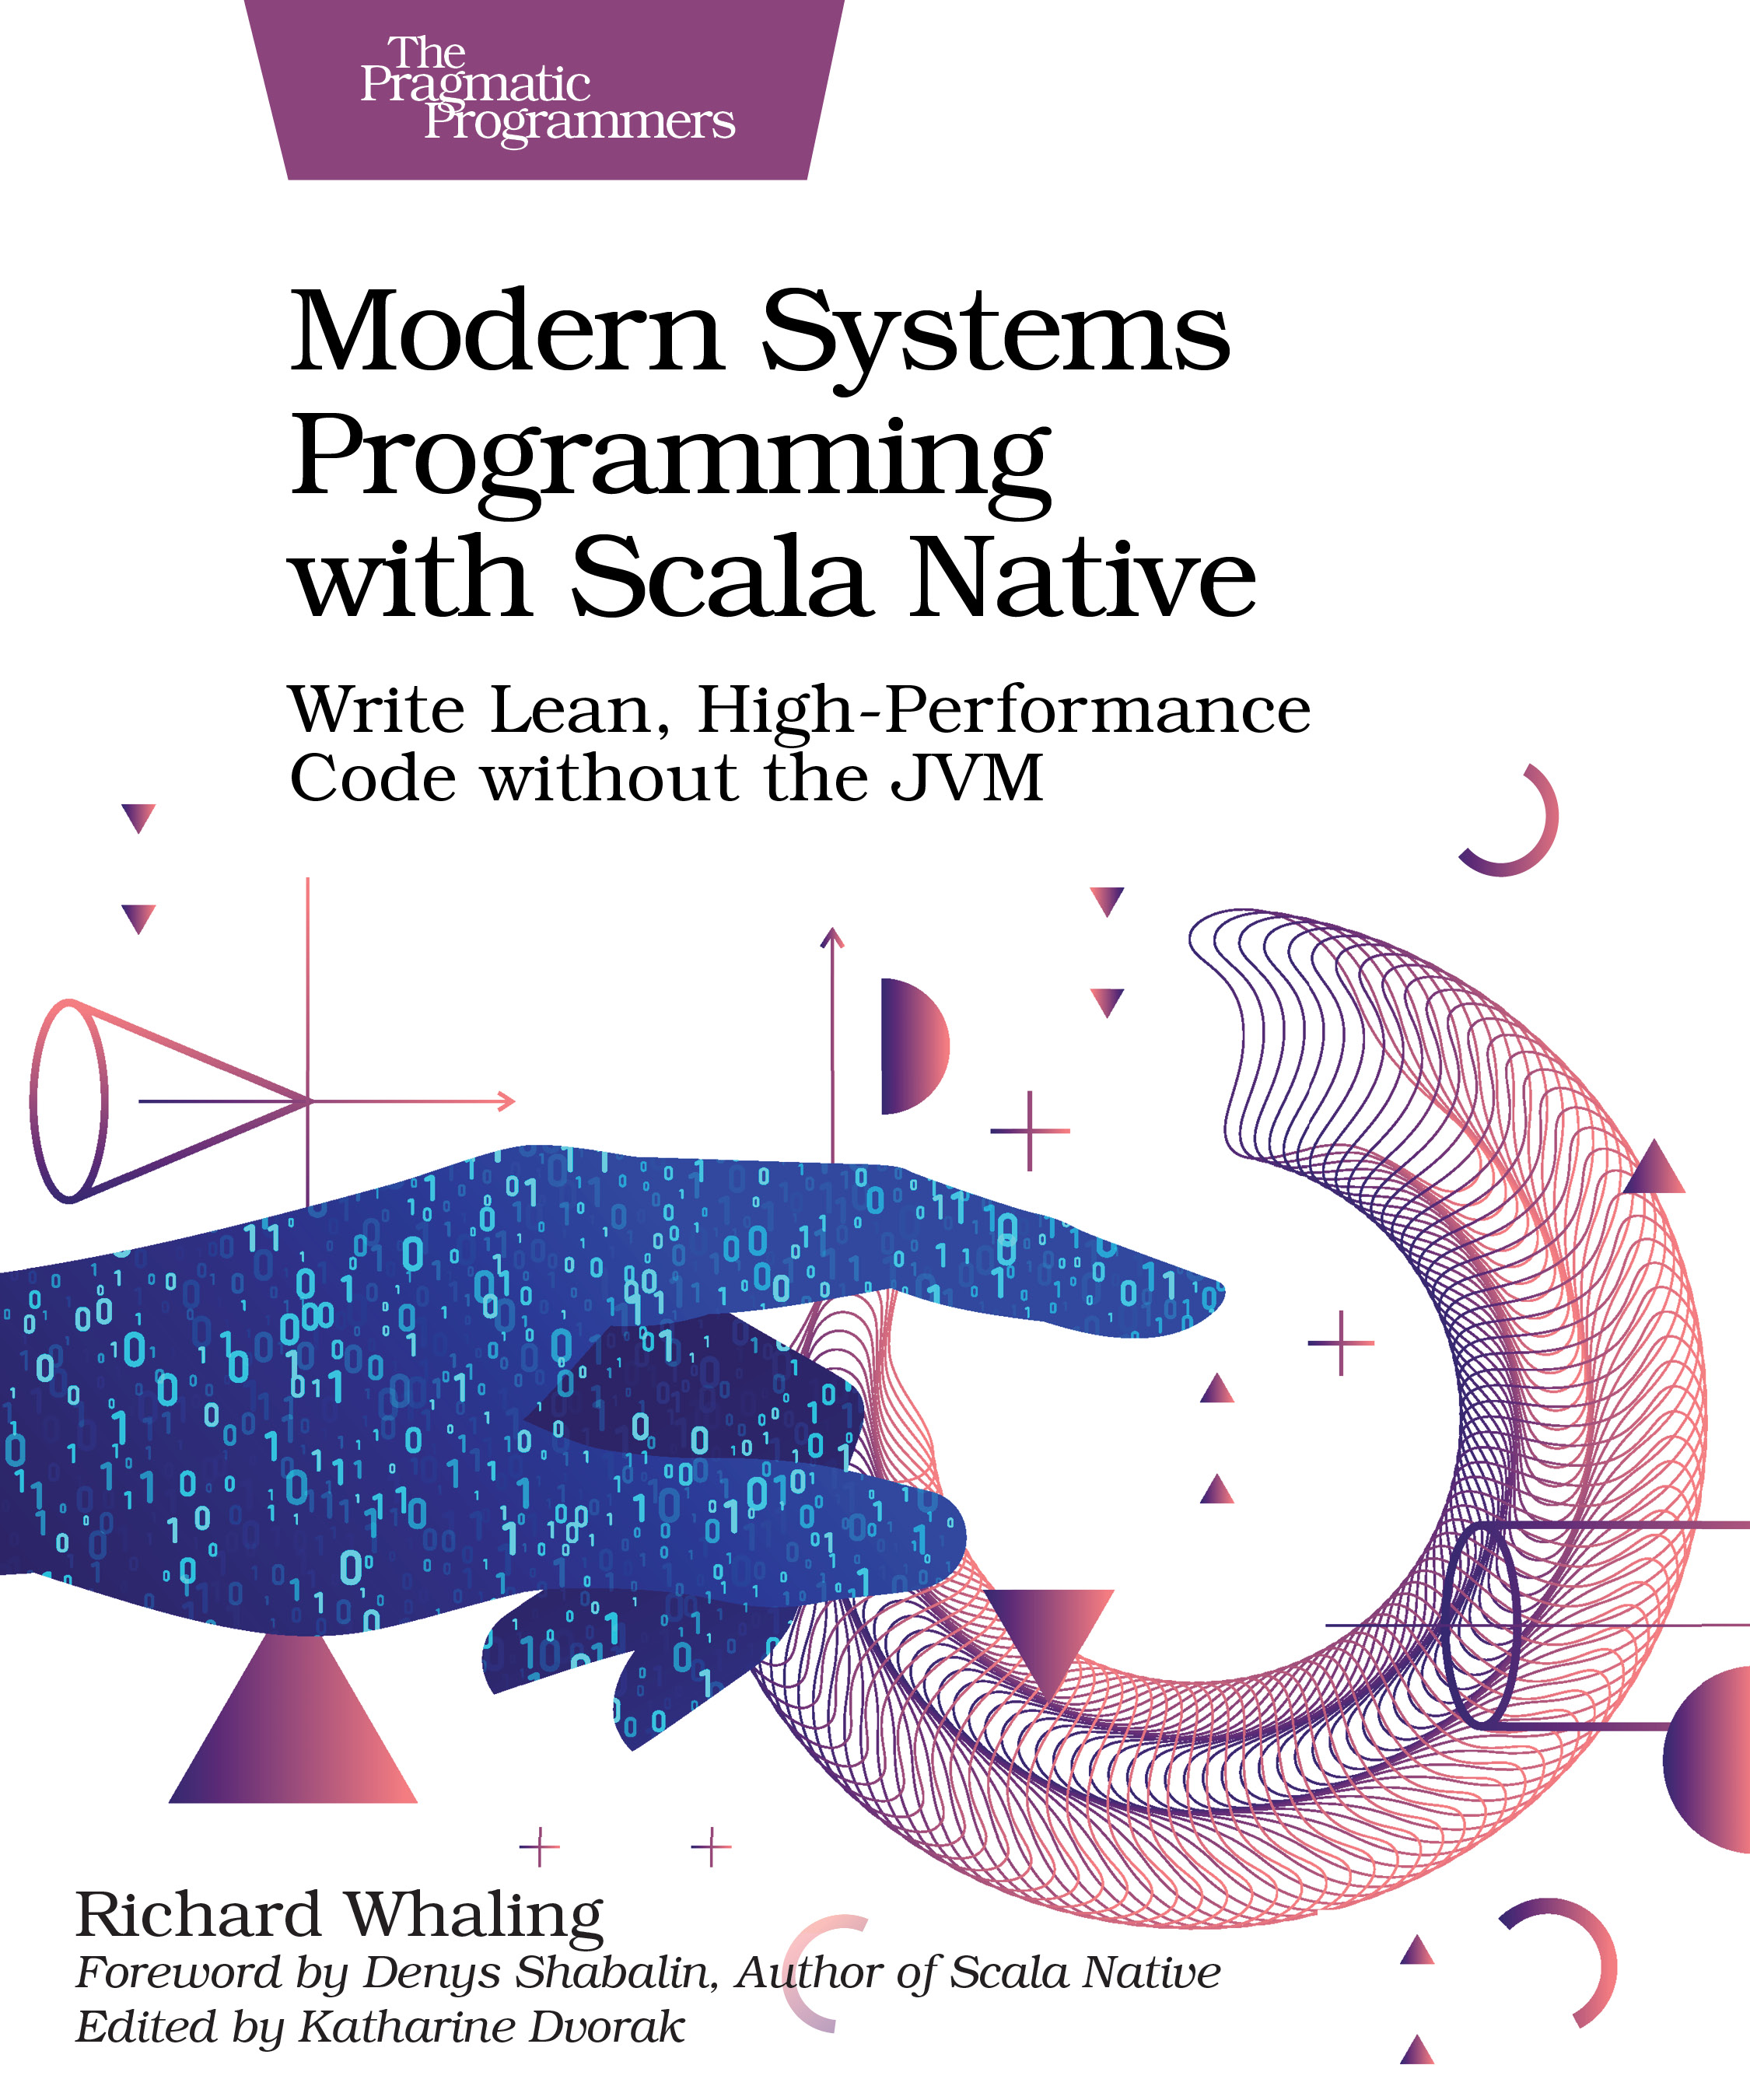
\includegraphics[width=7cm]{livro2020}
        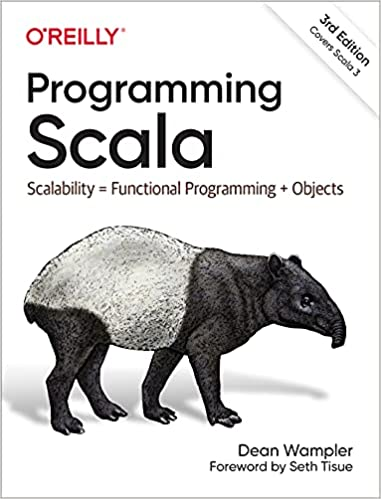
\includegraphics[width=7cm]{livro2021} \\
        {\tiny \sf Fonte: Autores }
    \end{center}
   \end{figure} 

	
	\begin{figure}[H]
		\centering
		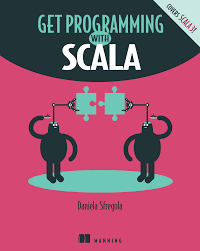
\includegraphics[width=7cm]{GetProgramming}
		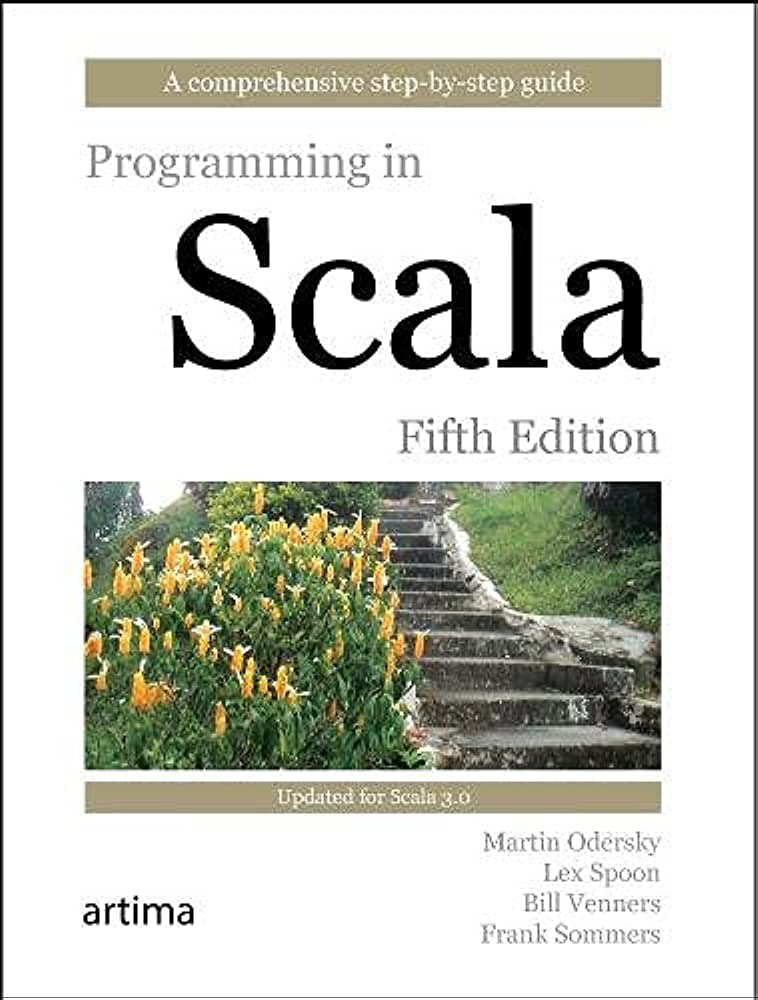
\includegraphics[width=7cm]{ProgrammingIn}
		\caption{}
		\label{fig:programming}
		Fonte: Autores
	\end{figure}

	\begin{figure}[H]
		\centering
		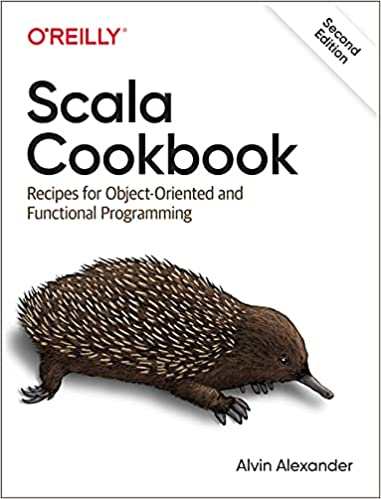
\includegraphics[width=7cm]{CookBook}
		\caption{}
		\label{fig:programming}
		Fonte: Autores
	\end{figure}

	